\section{Auswertung}
\label{sec:Auswertung}


Die Graphen werden sowohl mit Matplotlib \cite{matplotlib} als auch NumPy \cite{numpy} erstellt. Die Fehlerrechnung wird mithilfe von Uncertainties \cite{uncertainties} durchgeführt.\newline
\newline
Bei allen Messungen werden die Beschleunigungsspannung bei $U_.B=\SI{35}{\kilo\volt}$ und der Emissionsstrom bei $I_.E=\SI{1}{\milli\ampere}$ konstant eingestellt.

\subsection{Überprüfung der Bragg-Bedingung}
Der Kristallwinkel $\theta$ wird bei $\theta= \SI{14}{\degree}$ konstant gehalten, während der Winkel $\alpha$ des Geiger-Müller-Zählrohrs (GMZ) zwischen $\SI{26}{\degree}$ und $\SI{30}{\degree}$ mit einem Winkelzuwachs von $\Delta \alpha = \SI{0,1}{\degree}$ in $\Delta t = \SI{5}{\second}$ variiert wird.
Die aufgenommenen Messwerte sind in Tabelle \ref{tab:tab1} zu finden, der aufgezeichnete Graph ist in Abbildung \ref{fig:bragg}
Der Winkel bei dem das Maximum der Impulsrate $N$ erreicht ist, lässt sich ablesen zu $\alpha_.{max}=\SI{28,1}{\degree}$

\begin{table}
\centering
\caption{Die aufgenommenen Messwerte zur Überprüfung der Bragg-Bedingung.}
\label{tab:tabBragg1}
	\sisetup{table-format=1.2}
	\begin{tabular}{S[table-format=2.1]S[table-format=3.0]}
		\toprule
		{$\alpha/\si{\degree}$} & {$N/\si{1\per\second}$} \\
		\midrule
		26.0 &  28 \\
		26.1 &  38 \\
		26.2 &  37 \\
		26.3 &  33 \\
		26.4 &  34 \\
		26.5 &  35 \\
		26.6 &  43 \\
		26.7 &  45 \\
		26.8 &  43 \\
		26.9 &  58 \\
		27.0 &  57 \\
		27.1 &  68 \\
		27.2 &  71 \\
		27.3 &  86 \\
		27.4 & 100 \\
		27.5 &  97 \\
		27.6 &  99 \\
		27.7 & 126 \\
		27.8 & 119 \\
		27.9 & 131 \\
		28.0 & 130 \\
		\bottomrule
	\end{tabular}

\label{tab:tabBragg2}
	\sisetup{table-format=1.2}
	\begin{tabular}{S[table-format=2.1]S[table-format=3.0]}
		\toprule
		{$\alpha/\si{\degree}$} & {$N/\si{1\per\second}$} \\
		\midrule
		28.1 & 132 \\
		28.2 & 130 \\
		28.3 & 115 \\
		28.4 & 122 \\
		28.5 & 105 \\
		28.6 & 106 \\
		28.7 &  94 \\
		28.8 &  84 \\
		28.9 &  75 \\
		29.0 &  67 \\
		29.1 &  55 \\
		29.2 &  52 \\
		29.3 &  45 \\
		29.4 &  45 \\
		29.5 &  34 \\
		29.6 &  33 \\
		29.7 &  34 \\
		29.8 &  32 \\
		29.9 &  30 \\
		30.0 &  29 \\
		\bottomrule
	\end{tabular}

\label{tab:tab1}
\end{table}

\begin{figure}
\centering
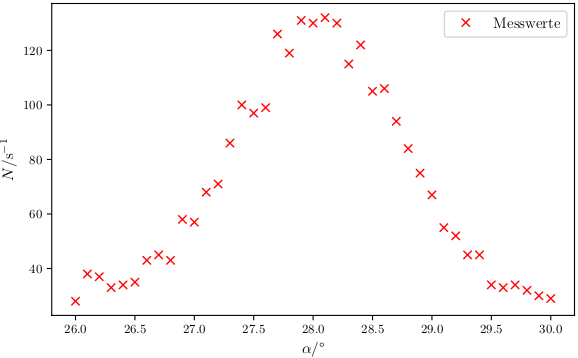
\includegraphics[width=\linewidth-70pt,height=\textheight-70pt,keepaspectratio]{content/images/bragg.png}
\caption{Die Impulsraten $N$ der Röntgenstrahlung für verschiedene Zählrohrwinkel $\alpha$ bei konstantem Kristallwinkel $\theta=\SI{14}{\degree}$.}
\label{fig:bragg}
\end{figure}

\subsection{Das Emissionsspektrum}

\subsubsection{Die minimale Wellenlänge}
In Abbildung \ref{fig:emission} ist das aufgenommene Emissionsspektrum der Röntgenröhre im Bereich von $\theta=\SI{4}{\degree}$ bis $\SI{26}{\degree}$ zu sehen.
Der Grenzwinkel lässt sich aus Abbildung \ref{fig:brems} ablesen zu
\[\theta_.{gr}=\SI{5}{\degree}\]
und damit die minimale Wellenlänge nach Formel \eqref{eq:lambda_min} zu
\[
\lambda_.{min}=\SI{35,1}{\pico\metre}\text{.}
\]
und die maximale kinetische Energie
\[
E_.{kin,max}=\SI{35316}{\eV}
\]
Die Literaturwerte berechnet sich mit der Elektronenladung $e_.0$, dem Planckschen Wirkungsquantum $h$ und der Lichtgeschwindigkeit im Vakuum $c$ zu
\[
\lambda_.{min,theo}=\frac{hc}{e_.0U_.B}=\SI{35,4}{\pico\metre}
\]
und
\[
E_.{max,theo}=e_.0U_.B=\SI{35000}{\eV}
\]

\begin{figure}
\centering
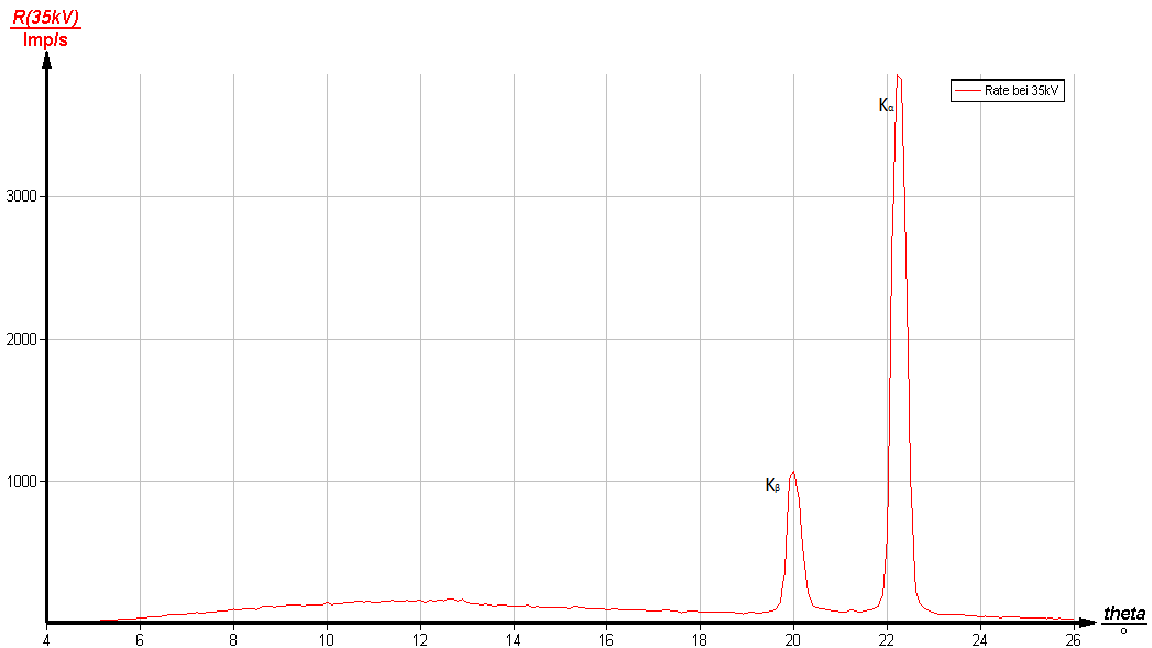
\includegraphics[width=\linewidth-70pt,height=\textheight-70pt,keepaspectratio]{content/images/Spektrum.png}
\caption{Die Impulsraten $N$ des Röntgenemissionsspektrums für verschiedene Kristallwinkel $\theta$.}
\label{fig:emission}
\end{figure}

\begin{figure}
\centering
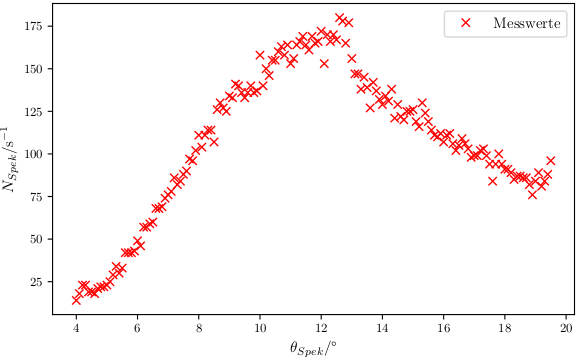
\includegraphics[width=\linewidth-70pt,height=\textheight-70pt,keepaspectratio]{content/images/konstSpektrum.png}
\caption{Der kontinuierliche Anteil des Röntgenemissionsspektrums.}
\label{fig:brems}
\end{figure}


\subsubsection{Das Auflösungsvermögen}

In Abbildung \ref{fig:Peak} ist eine Vergrößerung der Peaks der $K_.{\alpha}$- und $K_.{\beta}$-Linie zu sehen.
Zur Bestimmung der Halbwertsbreite werden die Werte für $\theta$ der Geraden
\begin{align*}
g_.1(\theta)&=\SI{6540}{s^{-1}\per\degree}\cdot\theta-\SI{129126}{s^{-1}}\text{,}\\
g_.2(\theta)&=\SI{-3990}{s^{-1}\per\degree}\cdot\theta+\SI{81082}{s^{-1}}
\end{align*}
gesucht, bei denen gilt $g_.{1/2}(\theta)=\frac{N_.{\alpha,max}}{2}=\SI{540}{s^{-1}}$\newline
und die, bei denen für die Geraden
\begin{align*}
g_.3(\theta)&=\SI{20140}{s^{-1}\per\degree}\cdot\theta-\SI{442454}{s^{-1}}\text{,}\\
g_.4(\theta)&=\SI{-15600}{s^{-1}\per\degree}\cdot\theta+\SI{352019}{s^{-1}}
\end{align*}
gilt $g_.{3/4}(\theta)=\frac{N_.{\beta,max}}{2}=\SI{1929}{s^{-1}}$.\newline
Daraus ergeben sich die Werte
\begin{align*}
\theta_.3&=\theta_.{\alpha-}=\SI{22,06}{\degree}\text{,}\\
\theta_.4&=\theta_.{\alpha+}=\SI{22,44}{\degree}\text{,}\\
\theta_.1&=\theta_.{\beta-}=\SI{19,83}{\degree}\text{,}\\
\theta_.2&=\theta_.{\beta+}=\SI{20,19}{\degree}
\end{align*}
und mit Gleichung \eqref{eq:E} für das Auflösungsvermögen
\begin{align*}
\Delta E_.{\alpha}&=\SI{130,7}{\eV}\\
\Delta E_.{\beta}&=\SI{155,0}{\eV}
\end{align*}

\begin{figure}
\centering
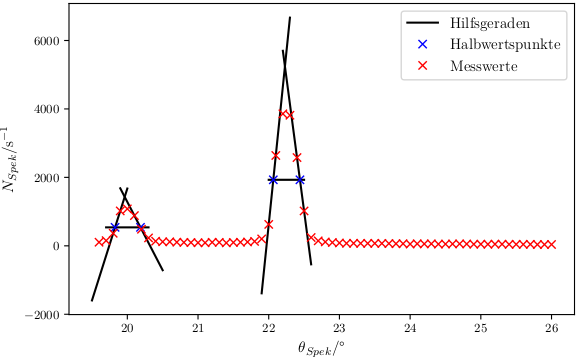
\includegraphics[width=\linewidth-70pt,height=\textheight-70pt,keepaspectratio]{content/images/PeakSpektrum.png}
\caption{Die Peaks der Impulsraten des Röntgenemissionsspektrums in der Nähe der $K_.{\alpha}$- und $K_.{\beta}$-Linie.}
\label{fig:Peak}
\end{figure}

\subsubsection{Die Abschirmkoeffizienten von Cu}

Die Maxima der $K_.{\alpha}$- und $K_.{\beta}$-Linie lassen sich aus \ref{fig:Peak} ablesen zu
\begin{align*}
\theta_.{\alpha,max}&=\SI{22,2}{\degree}\text{,}\\
\theta_.{\beta,max}&=\SI{20,0}{\degree}\text{.}
\end{align*}
Mit Gleichung \eqref{eq:E} ergeben sich so
\begin{align*}
E_.{K_.{\alpha}}&=\SI{8641}{\eV}\text{,}\\
E_.{K_.{\beta}}&=\SI{9000}{\eV}\text{.}
\end{align*}
Damit lassen sich nun die Abschirmkoeffizienten $\sigma_.K$,$\sigma_.L$ und $\sigma_.M$ mithilfe von Gleichung \eqref{eq:E_n} und der Kernladungszahl des Kupfers $z=29$ bestimmen zu
\begin{align*}
\sigma_.K&=z-\sqrt{\frac{E_.{K_.{\beta}}}{R_.{\inf}}}=3,28\text{,}\\
\sigma_.L&=z-\sqrt{\left(z-\sigma_.K\right)^2-\frac{E_.{K_.{\alpha}}}{R_.{\inf}}}=13,16\text{,}\\
\sigma_.M&=z-\sqrt{\left(z-\sigma_.K\right)^2-\frac{E_.{K_.{\beta}}}{R_.{\inf}}}=29
\end{align*}

\subsection{Das Absorptionsspektrum}
\subsubsection{Die $K$-Kanten von Atomen mit $30\leq z\leq 50$}
In den Tabellen \ref{tab:S_K} und den zugehörigen Graphen \ref{fig:Br} bis \ref{fig:Zr} sind die aufgenommenen Messwerte zur Bestimmung der $K$-Kanten von Brom, Strontium, Zink und Zirkonium zu finden.
Die Winkel bei denen sich die $K$-Kante befinden lassen sich ablesen zu
\begin{align*}
\theta_.{Br} &= \SI{13,4}{\degree}\text{,}\\
\theta_.{Sr} &= \SI{11,1}{\degree}\text{,}\\
\theta_.{Zn} &= \SI{18,6}{\degree}\text{,}\\
\theta_.{Zr} &= \SI{9,9}{\degree}\text{.}
\end{align*}
Daraus ergeben sich mit Gleichung \eqref{eq:E} die Energien
\begin{align*}
E_.{K_.{Br}} &= \SI{13282}{\eV}\text{,}\\
E_.{K_.{Sr}} &= \SI{15988}{\eV}\text{,}\\
E_.{K_.{Br}} &= \SI{9650}{\eV}\text{,}\\
E_.{K_.{Br}} &= \SI{17903}{\eV}\text{.}
\end{align*}
Die Abschirmkoeffizienten $\sigma_.K$ der Elemente lassen sich
mit den Kernladungszahlen
\begin{align*}
z_.{Br} &= 35\text{,}\\
z_.{Sr} &= 38\text{,}\\
z_.{Zn} &= 30\text{,}\\
z_.{Zr} &= 40
\end{align*}
über
\[
\sigma_.K =z - \sqrt{\frac{E_.K}{R_.{\inf}}}
\]
bestimmen zu
\begin{align*}
\sigma_.{K_.{Br}}&=3,75\text{,}\\
\sigma_.{K_.{Sr}}&=3,71\text{,}\\
\sigma_.{K_.{Zn}}&=3,36\text{,}\\
\sigma_.{K_.{Zr}}&=3,72\text{.}
\end{align*}

\begin{table}
\centering
\caption{Die aufgenommenen Messwerte zur Bestimmung des Abschirmkoeffizienten $\sigma_.K$ von Brom, Strontium, Zink und Zirkonium.}
\label{tab:tabBr}
	\sisetup{table-format=1.2}
	\begin{tabular}{S[table-format=2.1]S[table-format=3.0]}
		\toprule
		{$\theta_.{Br}/\si{\degree}$} & {$N/\si{1\per\second}$} \\
		\midrule
		12.2 &   9 \\
		12.3 &   9 \\
		12.4 &  10 \\
		12.5 &  10 \\
		12.6 &  10 \\
		12.7 &   9 \\
		12.8 &  12 \\
		12.9 &  12 \\
		13.0 &  17 \\
		13.1 &  18 \\
		13.2 &  22 \\
		13.3 &  22 \\
		13.4 &  23 \\
		13.5 &  21 \\
		13.6 &  18 \\
		13.7 &  20 \\
		13.8 &  17 \\
		13.9 &  18 \\
		14.0 &  18 \\
		14.1 &  17 \\
		14.2 &  17 \\
		\bottomrule
	\end{tabular}

\label{tab:tabSr}
	\sisetup{table-format=1.2}
	\begin{tabular}{S[table-format=2.1]S[table-format=3.0]}
		\toprule
		{$\theta_.{Sr}/\si{\degree}$} & {$N/\si{1\per\second}$} \\
		\midrule
		10.0 &  21 \\
		10.1 &  22 \\
		10.2 &  23 \\
		10.3 &  23 \\
		10.4 &  20 \\
		10.5 &  22 \\
		10.6 &  21 \\
		10.7 &  25 \\
		10.8 &  39 \\
		10.9 &  52 \\
		11.0 &  66 \\
		11.1 &  73 \\
		11.2 &  72 \\
		11.3 &  71 \\
		11.4 &  67 \\
		11.5 &  68 \\
		11.6 &  69 \\
		11.7 &  67 \\
		11.8 &  68 \\
		11.9 &  66 \\
		12.0 &  63 \\
		\bottomrule
	\end{tabular}

\label{tab:tabZn}
	\sisetup{table-format=1.2}
	\begin{tabular}{S[table-format=2.1]S[table-format=3.0]}
		\toprule
		{$\theta_.{Zn}/\si{\degree}$} & {$N/\si{1\per\second}$} \\
		\midrule
		17.6 &  31 \\
		17.7 &  32 \\
		17.8 &  31 \\
		17.9 &  34 \\
		18.0 &  30 \\
		18.1 &  32 \\
		18.2 &  31 \\
		18.3 &  36 \\
		18.4 &  47 \\
		18.5 &  50 \\
		18.6 &  59 \\
		18.7 &  57 \\
		18.8 &  54 \\
		18.9 &  55 \\
		19.0 &  58 \\
		19.1 &  54 \\
		19.2 &  56 \\
		19.3 &  54 \\
		19.4 &  57 \\
		19.5 &  57 \\
		19.6 &  65 \\
		\bottomrule
	\end{tabular}

\label{tab:tabZr}
	\sisetup{table-format=1.2}
	\begin{tabular}{S[table-format=2.1]S[table-format=3.0]}
		\toprule
		{$\theta_.{Zr}/\si{\degree}$} & {$N/\si{1\per\second}$} \\
		\midrule
		8.8 &  39 \\
		8.9 &  45 \\
		9.0 &  46 \\
		9.1 &  45 \\
		9.2 &  46 \\
		9.3 &  46 \\
		9.4 &  46 \\
		9.5 &  50 \\
		9.6 &  58 \\
		9.7 &  67 \\
		9.8 &  81 \\
		9.9 &  87 \\
		10.0 &  89 \\
		10.1 &  95 \\
		10.2 &  95 \\
		10.3 & 101 \\
		10.4 &  97 \\
		10.5 & 101 \\
		10.6 &  99 \\
		10.7 & 104 \\
		10.8 & 102 \\
		\bottomrule
	\end{tabular}

\label{tab:S_K}
\end{table}

\begin{figure}
\centering
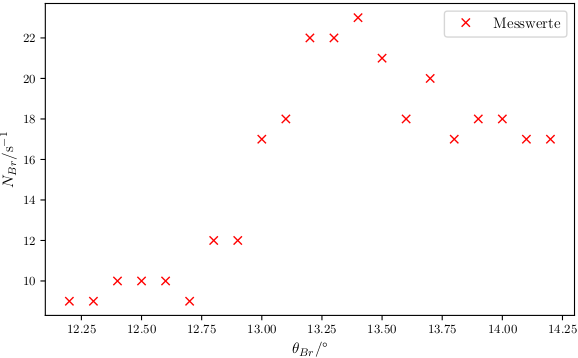
\includegraphics[width=\linewidth-70pt,height=\textheight-70pt,keepaspectratio]{content/images/Br.png}
\caption{Das Röntgenabsorptionsspektrum von Brom.}
\label{fig:Br}

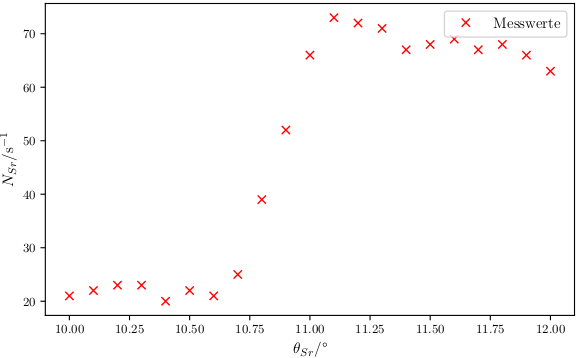
\includegraphics[width=\linewidth-70pt,height=\textheight-70pt,keepaspectratio]{content/images/Sr.png}
\caption{Das Röntgenabsorptionsspektrum von Strontium.}
\label{fig:Sr}
\end{figure}


\begin{figure}
\centering
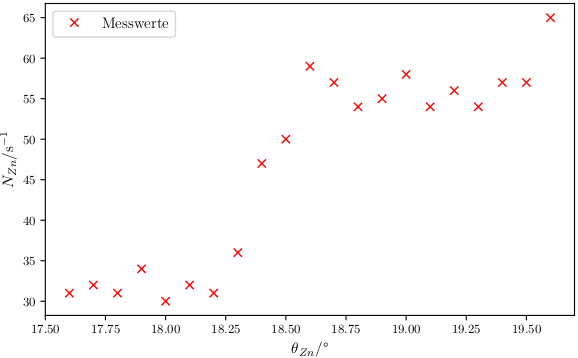
\includegraphics[width=\linewidth-70pt,height=\textheight-70pt,keepaspectratio]{content/images/Zn.png}
\caption{Das Röntgenabsorptionsspektrum von Zink.}
\label{fig:Zn}

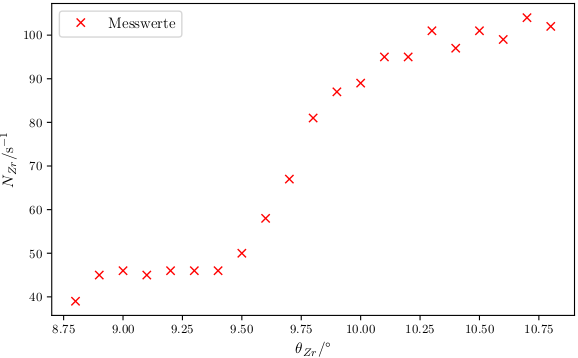
\includegraphics[width=\linewidth-70pt,height=\textheight-70pt,keepaspectratio]{content/images/Zr.png}
\caption{Das Röntgenabsorptionsspektrum von Zirkonium.}
\label{fig:Zr}
\end{figure}

\subsubsection{Das Moseley-Gesetz}
In Abbildung \ref{fig:Moseley} ist die Wurzel der Energien der $K$-Kante $E_.K$ gegen die Kernladungszahlen $z$ aufgetragen. Die lineare Regression $\sqrt{E_.K}(z)=az+b$ liefert die Parameter
\begin{align*}
a&=\SI{3,56(6)}{\sqrt{\eV}}\text{,}\\
b&=\SI{-8,7(21)}{\sqrt{\eV}}\text{.}
\end{align*}
Ein Koeffizientenvergleich mit dem Moseley-Gesetz für den Übergang vom 1. angeregten in den Grundzustand
\[
E_.K = R_.{\inf}z_.{eff}^2\cdot\frac{3}{4}
\]
liefert die Beziehung für die Rydbergenergie
\[
R_.{\inf}=\frac{3}{4}a^2=\SI{16,87(32)}{\eV}
\]
Der Fehler von $R_.{\inf}$ berechnet sich dabei mit dem bereits bekannten Fehler von $a$, $\sigma_.a$, über die Gaußsche Fehlerfortpflanzung zu
\[
\sigma_.R=\sqrt{\left(\frac{\partial R_.{\inf}}{\partial a}\right)^2\sigma^2_.a}=\frac{3}{2}a\sigma_.a
\]

\begin{figure}
\centering
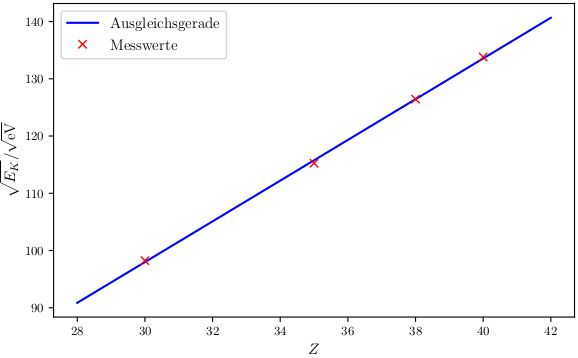
\includegraphics[width=\linewidth-70pt,height=\textheight-70pt,keepaspectratio]{content/images/Moseley.png}
\caption{Die Wurzel der Energien der $K$-Kanten in Abhängigkeit von der Kernladungszahl $z$.}
\label{fig:Moseley}
\end{figure}
\subsubsection{Die $L_.{II}$- und $L_.{III}$-Kante von Wismuth}
Die Werte zur Bestimmung der $L$-Kanten von Wismuth sind in Tabelle \ref{tab:Bi} und der zugehörige Graph in Abbildung \ref{fig:Bi} zu finden.
Die Winkel der Kanten lassen sich ablesen zu
\[
\theta_.{L_.{II}}=\SI{11,3}{\degree}\, \text{und}\, \theta_.{L_.{III}}=\SI{13,3}{\degree}
\]
Mit Gleichung \eqref{eq:E} ergeben sich die Energien
\[
E_.{L_.{II}}=\SI{15709}{\eV}\, \text{und}\, E_.{L_.{III}}=\SI{13380}{\eV}
\]
und damit
\[
\Delta E = \SI{2329}{\eV}\text{.}
\]
Mit der Sommerfeldschen Feinstrukturkonstante $\alpha$ und Gleichung \eqref{eq:sigma_L}
ergibt sich somit für den Abschirmkoeffizienten von Wismuth
\[
\sigma_.L=3,31
\]
Der Literaturwert ergibt sich mit $\Delta E=\SI{2292}{\eV}$\cite{Bi} zu
\[
\sigma_.L=3,58
\]

\begin{table}
\centering
\caption{Die aufgenommenen Messwerte zur Bestimmung des Abschirmkoeffizienten $\sigma_.L$ von Wismuth.}
\label{tab:tabBi1}
	\sisetup{table-format=1.2}
	\begin{tabular}{S[table-format=2.1]S[table-format=3.0]}
		\toprule
		{$\theta_.{Bi}/\si{\degree}$} & {$N/\si{1\per\second}$} \\
		\midrule
		10.0 &  40 \\
		10.1 &  41 \\
		10.2 &  42 \\
		10.3 &  43 \\
		10.4 &  43 \\
		10.5 &  42 \\
		10.6 &  47 \\
		10.7 &  49 \\
		10.8 &  51 \\
		10.9 &  49 \\
		11.0 &  50 \\
		11.1 &  56 \\
		11.2 &  61 \\
		11.3 &  61 \\
		11.4 &  61 \\
		11.5 &  60 \\
		11.6 &  59 \\
		11.7 &  59 \\
		11.8 &  55 \\
		11.9 &  56 \\
		12.0 &  57 \\
		12.1 &  60 \\
		12.2 &  54 \\
		\bottomrule
	\end{tabular}

\label{tab:tabBi2}
	\sisetup{table-format=1.2}
	\begin{tabular}{S[table-format=2.1]S[table-format=3.0]}
		\toprule
		{$\theta_.{Bi}/\si{\degree}$} & {$N/\si{1\per\second}$} \\
		\midrule
		12.3 &  51 \\
		12.4 &  52 \\
		12.5 &  48 \\
		12.6 &  48 \\
		12.7 &  46 \\
		12.8 &  46 \\
		12.9 &  51 \\
		13.0 &  54 \\
		13.1 &  61 \\
		13.2 &  66 \\
		13.3 &  67 \\
		13.4 &  65 \\
		13.5 &  65 \\
		13.6 &  60 \\
		13.7 &  64 \\
		13.8 &  63 \\
		13.9 &  59 \\
		14.0 &  59 \\
		14.1 &  56 \\
		14.2 &  55 \\
		14.3 &  59 \\
		14.4 &  53 \\
		14.5 &  54 \\
		\bottomrule
	\end{tabular}

\label{tab:Bi}
\end{table}

\begin{figure}
\centering
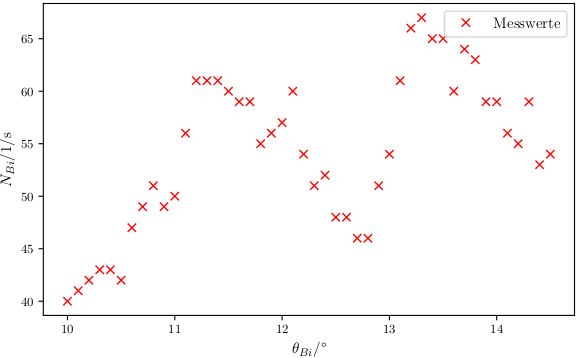
\includegraphics[width=\linewidth-70pt,height=\textheight-70pt,keepaspectratio]{content/images/Bi.png}
\caption{Das Röntgenabsorptionsspektrum von Wismuth.}
\label{fig:Bi}
\end{figure}
